	\section{Явление полного внутреннего отражения, его применения. Оптические элементы и
		приборы, работающие на явлении полного внутреннего отражения. Оптоволокно,
		типы оптоволокна.}
	Сначала наивное. Мы знаем формулу Снеллиуса $\sin \theta = n_{21} \sin \theta'$, где $n_{21}$ -- это относительная оптическая плотность. Если $n_{21} < 1$ то должен существовать такой угол падения $\arcsin n_{21}$ после которого не может уже существовать никакого прошедшего луча, а только отраженный. Так как свету некуда деться, кроме как отразиться, то он отражается полностью. 
	
	Теперь как это выглядит с точки зрения волновой оптики (Сивухин с 402)\\
	Пусть у нас есть падающая волна:
	\begin{align*}
		E^{e} = \mathcal{E} e^{i(\omega t - k_1 r)}
	\end{align*}
	Мы из соображений геометрической оптики знаем, что должны быть еще отраженная (r) и прошедшая (d) волны:
	\begin{align*}
	E^{r} = \mathcal{R} e^{i(\omega t - k'_1 r)}\\E^{d} = \mathcal{D} e^{i(\omega t - k_2 r)}
	\end{align*}
	Мы предполагаем что они тоже плоские из соображений симметрии. Равенство частот у всех трех объясняется тем, что напряженности могут иметь только гармоническую зависимость от времени, а в случае наложения двух плоских полей с разными частотами такое не выполняется.\\
	Из соотношений симметрии надо заключить, что касательная к плоскости составляющая волнового вектора у всех трех волн одинаковая. В нашем случае это проекция на ось x (смотри рисунок)
	\begin{figure}[H]
		\includegraphics*[scale = 0.3]{2_1}
	\end{figure}
	То есть: $k_{1x} = k'_{1x} = k_{2x}$\\
	Так же можем написать про волновые вектора:
	\begin{align*}
	k_1^2 = k_1'^2 = \dfrac{\omega^2 }{c^2 } \varepsilon_1\\
	k_2^2 = \dfrac{\omega^2 }{c^2 } \varepsilon_2
	\end{align*}
	Где эпсилон 1 и 2 это диэлектрическая проницаемость среды из которой пришел луч и в которую ушел соответственно. Отсюда можно узнать их z составляющие:
	\begin{align*}
	k'_{1z} = - \sqrt{k_1^2 - k_{1x}^2}\\
	k_{2z} = \sqrt{k_2^2 - k_{1x}^2}	
	\end{align*}
	Так как нас волнует полное внутреннее отражение, то рассмотрим случай, когда $k_2^2 < k_{1x}^2 $ так как $k_{1x} = k_1 \sin \phi$, то это условие равносильно условию $\sin \phi > \sqrt{\dfrac{\varepsilon_2}{\varepsilon_1}} = n_{21}$ так же как в геометрической оптике. Естественно чтобы такое условие вообще могло выполняться надо чтобы $n_{21}<1$. В этом случае $k_{2z}$ комплексный. Обозначим так: $k_{2z} = \dfrac{-i}{2h}$ Почему минус? Потому что корень это функция многозначная и нужную ветвь мы выбираем исходя из физических требований, а тут нужен как раз минус. Со всем этим можем написать отраженную волну как:
	\begin{align*}
	E^{d} = \mathcal{D}e^{-z/2h} e^{i(\omega t - k_{1x} x)}\\
	h = \dfrac{\lambda_1}{4\pi \sqrt{\sin^2 \phi  - n_{21}^2}}
	\end{align*}
	То есть волна идет вдоль границы, но затухает вглубь вещества (см рисунок)
	\begin{figure}[H]
		\centering
		\caption{Опыт Мандельштама и Селени}
		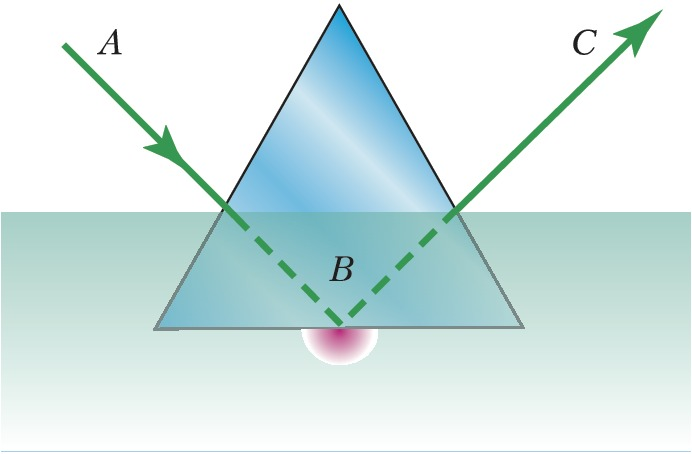
\includegraphics[scale = 1]{2_2}
	
	\end{figure}
	Эффект полного внутреннего отражения используется например в уголковых отражателях и во многих других призмах:
		\begin{figure}[H]
			\centering
			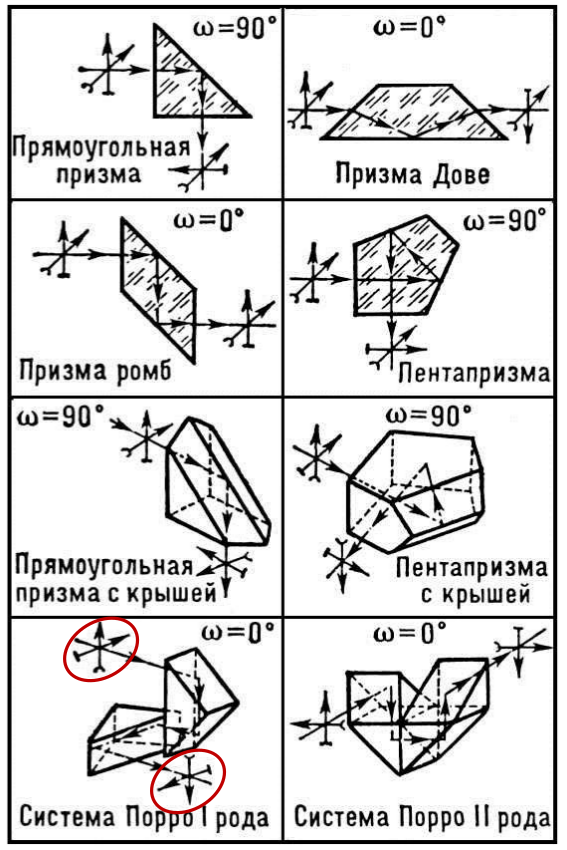
\includegraphics[scale = 0.3]{2_3}
		\end{figure}
	Оптоволокно это такая штука, в которой свет постоянно испытывает отражения от стенок. Состоит из двух слоев очевидно. Внешний имеет оптическую плотность больше. Заодно он защищает внутренний слой от повреждений. Сгибать сильно нельзя.